\documentclass[11pt,a4paper]{article}

\usepackage[spanish,es-nodecimaldot,es-tabla]{babel}
\usepackage{fontspec}
\usepackage{amsmath}
\usepackage{siunitx}
\usepackage{booktabs}
\usepackage{graphicx}
\usepackage{float}
\usepackage[font=small,labelfont=bf]{caption}
\usepackage[margin=2.4cm]{geometry}
\usepackage{microtype}
\usepackage[hidelinks]{hyperref}

\sisetup{output-decimal-marker={.}, separate-uncertainty=true}
\graphicspath{{../resultados/}}

\title{Astronomía para Todos\\[4pt]\large Taller 7: rotación del Sol a partir del análisis de las manchas solares}
\author{Sebastian Velandia Acevedo y Jesus Martinez}
\date{12 de noviembre de 2026}

\begin{document}
\maketitle

\section*{Datos y método}
Se usaron 26 imágenes reales del SDO, una por día a las 12:00 UT entre el 25 de noviembre y el 20 de diciembre de 2014,
tomadas por el instrumento HMI en el continuo visible (intensitygrama), descargadas de Helioviewer con norte solar arriba
y escala de \SI{2.4}{\arcsecond/px}.
Con un script en Python (\texttt{taller7/scripts/track\_sunspots.py}) en cada imagen se encontró el borde del disco,
se detectaron las regiones más oscuras que el entorno (las manchas), se agruparon y se convirtió la posición de cada grupo
en latitud $b$ y longitud $L$ heliográficas, corrigiendo la inclinación $B_0$ del eje solar
(entre $\ang{-1.6}$ y $\ang{+1.6}$ en este periodo). Luego se siguió cada grupo de un día al siguiente.
Se descartaron las manchas a menos de $0.08\,R_\odot$ del borde, donde el escorzo deforma la posición.

\begin{figure}[H]
\centering
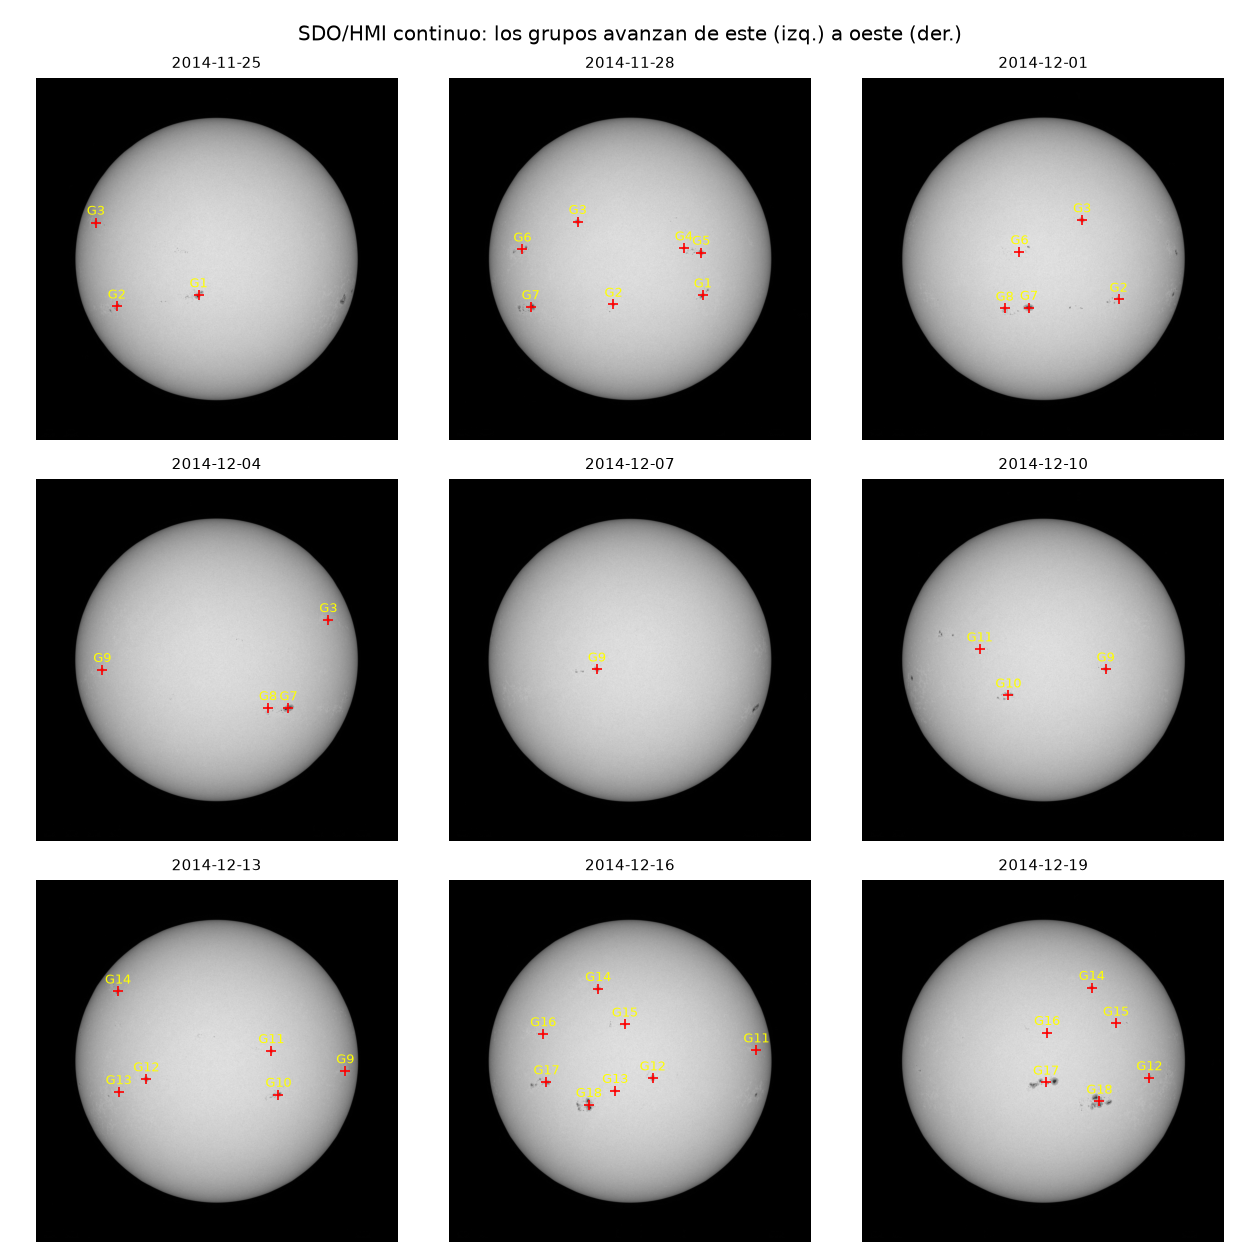
\includegraphics[width=0.92\textwidth]{mosaico_seguimiento.png}
\caption{Nueve de las 26 imágenes SDO/HMI (cada tres días). Las cruces marcan los grupos seguidos (G1--G18).
Todos avanzan de izquierda (borde este) a derecha (borde oeste).}
\end{figure}

% =====================================================================
\section{Actividad 1: comprobación de una hipótesis}

\textbf{H4 (propuesta):} las manchas son defectos o polvo en la óptica del telescopio (o fenómenos en la atmósfera terrestre)
y no pertenecen al Sol.

Con una imagen diaria durante 11 años se comprobaría cada hipótesis así:

\paragraph{H1 (cuerpos que orbitan el Sol).}
Un planeta o asteroide sería un objeto sólido y opaco: su forma y tamaño no cambiarían, se vería como un disco negro y nítido,
y se movería con un periodo orbital fijo (tercera ley de Kepler) que no depende de la latitud en la que aparece.
Además, al estar delante del Sol, su paso de un borde al otro tardaría lo mismo cerca del borde que del centro
(velocidad aparente constante) y el mismo objeto reaparecería con exactamente el mismo aspecto en cada tránsito, como Mercurio o Venus.
Si en cambio las manchas nacen, cambian de forma y desaparecen en días, y se ven \emph{comprimidas} cerca del borde,
H1 queda descartada.

\paragraph{H2 (nubes movidas por corrientes).}
Las nubes se moverían de forma desordenada: unas más rápido, otras más lento, en direcciones distintas, y cambiarían de dirección
según las corrientes. Se compararía la dirección y la velocidad de muchas manchas en el mismo día: si todas se desplazan
en la misma dirección, de forma paralela al ecuador y a una velocidad que solo depende de la latitud, no son nubes arrastradas al azar.

\paragraph{H3 (rasgos de la superficie que giran con el Sol).}
Si las manchas están pegadas a la superficie de una esfera que gira, entonces todas deben moverse en la misma dirección
(este $\to$ oeste), sus trayectorias deben ser paralelas al ecuador solar, deben verse más lentas y más estrechas cerca del borde
(escorzo) y más rápidas en el centro, y un grupo de vida larga debe reaparecer por el borde este unos 27 días después de
haberse ocultado. Con 11 años de imágenes también se vería que el periodo es el mismo año tras año.

\paragraph{H4 (defectos del instrumento o atmósfera terrestre).}
Un defecto en la óptica se quedaría quieto en la imagen (no cruzaría el disco) y no aparecería en otros telescopios;
algo en la atmósfera de la Tierra se movería en minutos, no en días, y el SDO ni siquiera mira a través de ella. Comparar con otro observatorio
(por ejemplo SOHO o un telescopio en tierra) y ver que la mancha está en el mismo sitio del disco descarta H4.

% =====================================================================
\section{Actividad 2: análisis de las imágenes del SDO}

\paragraph{1) ¿En qué dirección se mueven las manchas? ¿Todas en la misma?}
Todas se mueven de izquierda a derecha en la imagen, es decir, del borde \textbf{este} al borde \textbf{oeste} del Sol,
en trayectorias casi paralelas al ecuador solar. Las 18 manchas o grupos seguidos se movieron en la misma dirección
(en la figura~\ref{fig:lon} todas las rectas tienen pendiente positiva); ninguna se movió hacia la izquierda, ni hacia arriba o abajo
(la latitud de cada grupo cambió menos de $\ang{1}$ durante todo su recorrido).

\paragraph{2) ¿Parecen moverse aleatoriamente o todas juntas?}
Todas juntas, como un conjunto: las rectas de la figura~\ref{fig:lon} son prácticamente paralelas. Además se mueven más rápido
cuando pasan por el centro del disco y más despacio cerca de los bordes, que es justo lo que se espera de puntos fijos en una esfera
que gira vista de frente. No hay movimiento aleatorio.

\paragraph{3) ¿Se mueven con la misma velocidad?}
En velocidad angular (grados de longitud por día) son casi iguales: entre 12.8 y \SI{13.7}{\degree/día} para 17 de los 18 grupos
(tabla~\ref{tab:grupos}). Pero no son idénticas: los grupos cercanos al ecuador ($|b|<\ang{10}$) giran un poco más rápido que los
de latitud alta (el grupo G14, a $\ang{+30}$, es el más lento, con \SI{12.76}{\degree/día}). Esto es la \textbf{rotación diferencial}
del Sol (figura~\ref{fig:dif}). En velocidad lineal sobre la imagen (píxeles por día) tampoco son iguales: son mayores en el centro
del disco que cerca de los bordes, por efecto de la perspectiva.

\paragraph{4) ¿Por qué H1 y H2 no son buenas hipótesis?}
\textbf{H1:} las manchas cambian de forma y tamaño, aparecen y desaparecen en pocos días (por ejemplo, G17 y G18 crecieron mucho entre
el 14 y el 19 de diciembre) y se ven aplastadas cerca del borde. Un cuerpo sólido que orbita no hace eso. Además, todas las manchas de
todas las latitudes tienen casi el mismo periodo; si fueran planetas a distintas distancias tendrían periodos muy diferentes
(tercera ley de Kepler), y nunca se ha visto pasar un ``planeta'' así fuera del disco.
\textbf{H2:} si fueran nubes llevadas por corrientes, se moverían en direcciones distintas y con velocidades al azar. En cambio
todas van en la misma dirección, paralelas al ecuador, con una velocidad que solo depende de la latitud y que se mantiene constante
durante más de una semana (residuos menores a $\ang{1}$ respecto de una recta). Eso indica un movimiento de conjunto: la rotación del Sol (H3).

% =====================================================================
\section{Estimación del periodo de rotación solar}

\paragraph{5) Método.}
\begin{enumerate}
\item Elegir una mancha (o grupo) fácil de reconocer que aparezca en varias imágenes seguidas.
\item En cada imagen medir el centro y el radio $R$ del disco y la posición $(x,y)$ de la mancha.
\item Convertir esa posición en longitud $L$ respecto al meridiano central:
  $\sin L = \dfrac{x}{R\cos b}$, con $\sin b = y/R$ (latitud), corrigiendo por $B_0$ si se quiere más precisión.
  Este paso es clave: en la imagen la mancha \emph{parece} frenar cerca de los bordes, pero en longitud avanza a ritmo constante.
\item Graficar $L$ contra el tiempo y ajustar una recta: la pendiente $\omega$ es la velocidad angular en grados por día.
\item El periodo visto desde la Tierra (sinódico) es $T_{\text{sin}} = \ang{360}/\omega$.
\item Como la Tierra avanza en su órbita en el mismo sentido (unos \SI{1.0}{\degree/día}), el periodo real o sideral es
  $\dfrac{1}{T_{\text{sid}}} = \dfrac{1}{T_{\text{sin}}} + \dfrac{1}{\SI{365.25}{d}}$.
\item Repetir con muchas manchas y promediar.
\end{enumerate}

\emph{Ejemplo a mano (grupo G9, latitud $\ang{-4}$):} el 4 de diciembre estaba en $L=\ang{-54.2}$ y el 13 de diciembre en $L=\ang{+65.8}$.
Recorrió $\ang{120.0}$ en 9 días, o sea $\omega=\SI{13.33}{\degree/día}$, y $T_{\text{sin}}=360/13.33=\SI{27.0}{días}$.
Un método aún más simple, al estilo de Galileo, es contar los días que tarda una mancha en cruzar de un borde al otro
(media vuelta, $\approx 13.5$ días) y multiplicar por 2.

\begin{figure}[H]
\centering
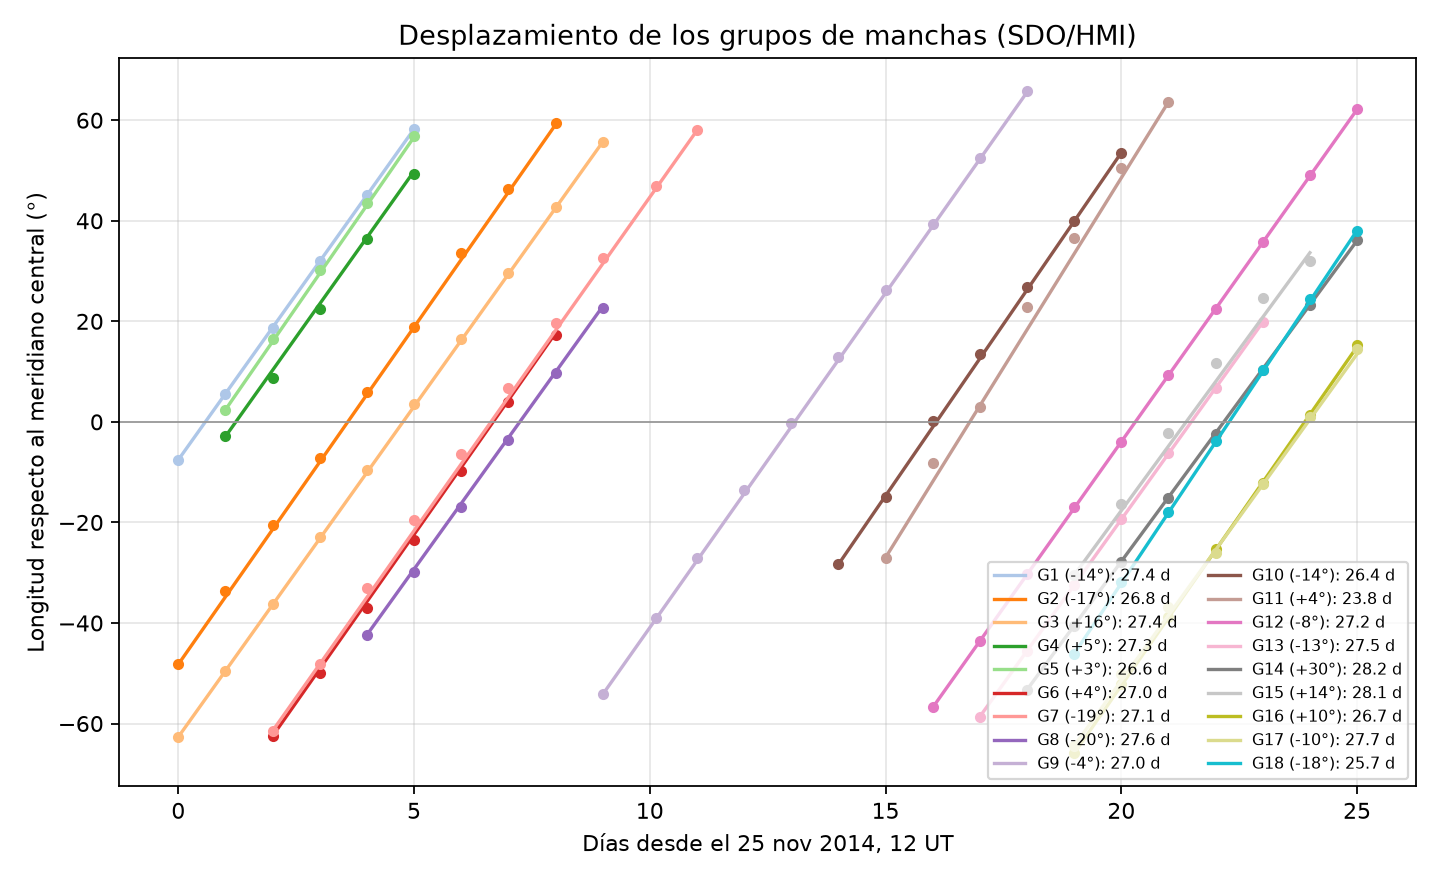
\includegraphics[width=0.95\textwidth]{longitud_vs_tiempo.png}
\caption{Longitud respecto al meridiano central contra tiempo para los 18 grupos seguidos (puntos) y su ajuste lineal (rectas).
La pendiente es la velocidad angular sinódica; en la leyenda va la latitud y el periodo sinódico de cada grupo.}
\label{fig:lon}
\end{figure}

\paragraph{6) Periodo de rotación con las imágenes SDO.}
\begin{table}[H]
\centering
\caption{Resultados por grupo de manchas. $\omega$: velocidad angular sinódica; $T_{\text{sid}}$: periodo sideral.}
\label{tab:grupos}
\small
\begin{tabular}{lllrrrr}
\toprule
Grupo & Primer día & Último día & $b$ (°) & $\omega$ (°/día) & $T_{\text{sin}}$ (d) & $T_{\text{sid}}$ (d) \\
\midrule
G1  & 25 nov & 30 nov & $-13.7$ & $13.16 \pm 0.01$ & 27.4 & 25.4 \\
G2  & 25 nov & 3 dic  & $-17.0$ & $13.41 \pm 0.06$ & 26.8 & 24.9 \\
G3  & 25 nov & 4 dic  & $+16.4$ & $13.15 \pm 0.02$ & 27.4 & 25.4 \\
G4  & 26 nov & 30 nov & $+5.4$  & $13.19 \pm 0.22$ & 27.3 & 25.3 \\
G5  & 26 nov & 30 nov & $+3.5$  & $13.56 \pm 0.11$ & 26.6 & 24.7 \\
G6  & 27 nov & 3 dic  & $+4.0$  & $13.36 \pm 0.09$ & 27.0 & 25.0 \\
G7  & 27 nov & 6 dic  & $-19.4$ & $13.27 \pm 0.10$ & 27.1 & 25.2 \\
G8  & 29 nov & 4 dic  & $-20.0$ & $13.06 \pm 0.07$ & 27.6 & 25.6 \\
G9  & 4 dic  & 13 dic & $-3.9$  & $13.31 \pm 0.03$ & 27.0 & 25.1 \\
G10 & 9 dic  & 15 dic & $-14.3$ & $13.65 \pm 0.11$ & 26.4 & 24.6 \\
G11$^*$ & 10 dic & 16 dic & $+3.9$ & $15.10 \pm 0.41$ & 23.8 & 22.3 \\
G12 & 11 dic & 20 dic & $-7.9$  & $13.22 \pm 0.01$ & 27.2 & 25.3 \\
G13 & 12 dic & 18 dic & $-13.1$ & $13.07 \pm 0.01$ & 27.5 & 25.6 \\
G14 & 13 dic & 20 dic & $+29.7$ & $12.76 \pm 0.02$ & 28.2 & 26.1 \\
G15 & 14 dic & 19 dic & $+14.2$ & $12.82 \pm 0.58$ & 28.1 & 26.0 \\
G16 & 14 dic & 20 dic & $+10.3$ & $13.48 \pm 0.03$ & 26.7 & 24.8 \\
G17 & 14 dic & 20 dic & $-9.7$  & $12.99 \pm 0.16$ & 27.7 & 25.7 \\
G18 & 14 dic & 20 dic & $-18.4$ & $14.03 \pm 0.05$ & 25.7 & 23.9 \\
\bottomrule
\end{tabular}

\smallskip
\footnotesize $^*$G11 es un grupo pequeño y débil que cambió mucho de forma; su valor se aparta de los demás.
\end{table}

Promediando los 18 grupos (pesando por la incertidumbre de cada ajuste):
\[
\omega_{\text{sin}} = \SI{13.29 \pm 0.12}{\degree/día}
\quad\Rightarrow\quad
\boxed{T_{\text{sin}} \approx \SI{27.1 \pm 0.3}{días}}
\]
y corrigiendo por el movimiento orbital de la Tierra en diciembre (\SI{1.015}{\degree/día}):
\[
\omega_{\text{sid}} = \SI{14.30}{\degree/día}
\quad\Rightarrow\quad
\boxed{T_{\text{sid}} \approx \SI{25.2 \pm 0.3}{días}}
\]
La mediana da casi lo mismo (27.2 y 25.3 días), así que el resultado no depende del grupo atípico G11.

\begin{figure}[H]
\centering
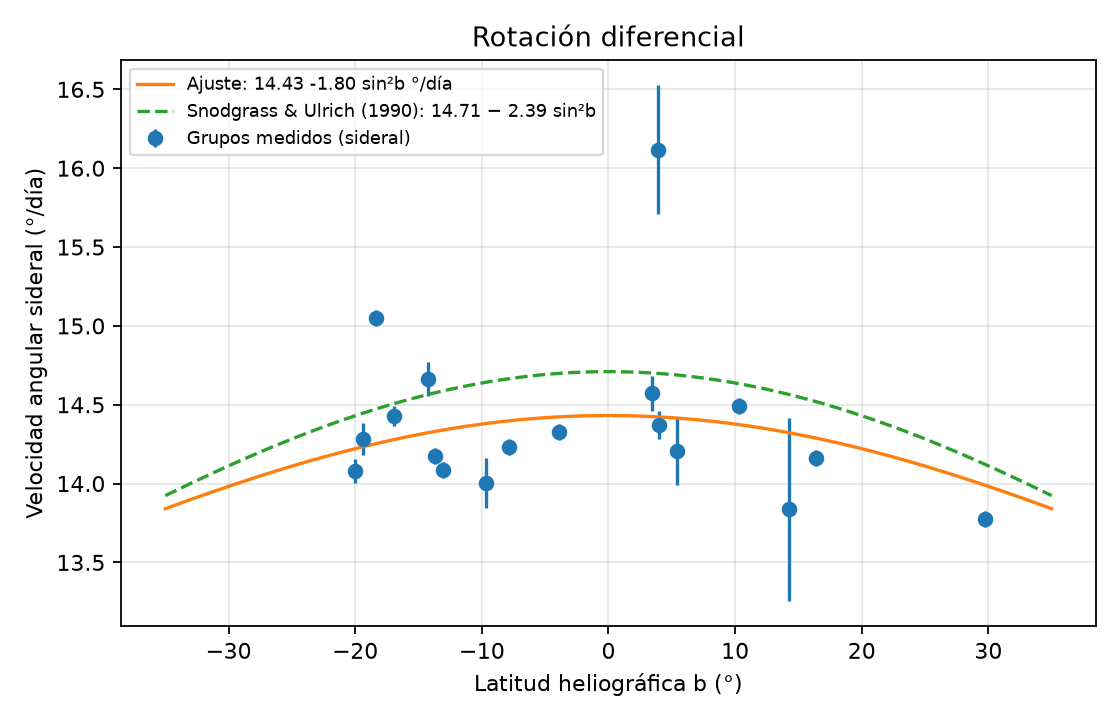
\includegraphics[width=0.75\textwidth]{rotacion_diferencial.png}
\caption{Velocidad angular sideral de cada grupo contra su latitud. El ajuste
$\omega = A + B\sin^2 b$ da $A = \SI{14.43}{\degree/día}$ (periodo ecuatorial de \SI{24.9}{días}) y $B=\SI{-1.8}{\degree/día}$:
el ecuador gira más rápido que las latitudes altas, en acuerdo con la curva de referencia de Snodgrass y Ulrich (1990).}
\label{fig:dif}
\end{figure}

\paragraph{7) ¿Qué tan confiable es el resultado?}
Es bastante confiable. El periodo sinódico de 27.1 días coincide con el valor de referencia de unos 27 días que da la guía
(y el sideral de 25.2 días con los $\approx 25$ días del ecuador solar que se reportan en la literatura); la diferencia es menor al 1~\%.
Lo que lo hace confiable es que se usaron 18 grupos distintos, en ambos hemisferios, con 5 a 10 imágenes cada uno, y que cada ajuste
lineal tiene residuos menores a un grado. Las limitaciones son:
\begin{itemize}
\item \textbf{Rotación diferencial:} no existe un solo periodo; depende de la latitud (de $\approx 24.9$ días sideral en el ecuador a
  $\approx 26$ días a $\ang{30}$). Nuestro promedio corresponde a latitudes de $\ang{0}$ a $\ang{20}$, donde están casi todas las manchas.
\item \textbf{Las manchas cambian:} crecen, se fragmentan y se desplazan un poco por sí mismas (movimientos propios), lo que cambia su
  centro de un día a otro (por eso G11 y G18 dan valores distintos).
\item \textbf{Cerca del borde} la posición se mide mal por el escorzo; por eso se descartaron esas detecciones.
\item \textbf{Resolución temporal y duración:} con una imagen diaria y solo 26 días, ningún grupo se siguió una vuelta completa;
  el periodo se extrapola de 5 a 10 días de movimiento.
\item Hay que distinguir el periodo \emph{sinódico} (visto desde la Tierra) del \emph{sideral}; olvidar esa corrección
  introduce un error de casi 2 días.
\end{itemize}

\section*{Conclusión}
Las manchas solares se mueven todas en la misma dirección, juntas y a ritmo constante en longitud, como lo harían puntos fijos sobre una
esfera que gira: el Sol rota sobre su eje (H3). Con las imágenes del SDO se obtuvo un periodo de \textbf{27.1 días visto desde la Tierra}
y de \textbf{25.2 días sideral}, y además se detectó que el ecuador gira más rápido que las latitudes altas.

\end{document}
